\documentclass[landscape]{article}

\usepackage[T1]{fontenc}

\usepackage[margin=0.5cm]{geometry}

\usepackage{tikz}

\usetikzlibrary{positioning,fit,calc,arrows.meta}



\definecolor{classhead}{RGB}{210,210,235}

\definecolor{classbody}{RGB}{235,235,248}

\definecolor{classborder}{RGB}{120,120,170}



\tikzset{
  umlclass/.style={draw=classborder, fill=classbody, rounded corners=1pt,
    minimum width=#1, text width=#1-6pt, align=center, font=\scriptsize, inner sep=2pt},
  umlclass/.default=2.8cm,
  classhead/.style={draw=classborder, fill=classhead,
    minimum width=#1, text width=#1-6pt, align=center, font=\scriptsize\bfseries, inner sep=2pt},
  classhead/.default=2.8cm,
  enumbox/.style={draw=classborder, fill=classbody, rounded corners=1pt,
    minimum width=#1, text width=#1-6pt, align=center, font=\scriptsize, inner sep=2pt},
  enumbox/.default=2.6cm,
  enumhead/.style={draw=classborder, fill=classhead,
    minimum width=#1, text width=#1-6pt, align=center, font=\scriptsize\bfseries, inner sep=2pt},
  enumhead/.default=2.6cm,
  assoc/.style={->, >=latex, draw=black!80, thin},
  compose/.style={->, >=latex, draw=black!80, thin},
  realize/.style={-{Triangle[open]}, draw=black!80, thin, dashed},
  dep/.style={->, >=latex, draw=black!80, thin, dashed},
  line/.style={draw=black!80, thin}
}



\newcommand{\umlNode}[6]{%
  \node[classhead=#3, anchor=north] (#1-head) at (#2) {#4};
  \node[umlclass=#3, anchor=north] (#1-attr) at (#1-head.south) {\vspace{1pt}#5\vspace{1pt}};
  \node[umlclass=#3, anchor=north] (#1-op) at (#1-attr.south) {\vspace{1pt}#6\vspace{1pt}};
  \node[fit=(#1-head)(#1-attr)(#1-op), inner sep=0pt] (#1) {};
}
\newcommand{\umlInterface}[6]{%
  \node[classhead=#3, anchor=north] (#1-head) at (#2) {%
    \textit{*\tiny$\langle\langle$interface$\rangle\rangle$*}\\[-2pt]#4};
  \node[umlclass=#3, anchor=north] (#1-attr) at (#1-head.south) {\vspace{1pt}#5\vspace{1pt}};
  \node[umlclass=#3, anchor=north] (#1-op) at (#1-attr.south) {\vspace{1pt}#6\vspace{1pt}};
  \node[fit=(#1-head)(#1-attr)(#1-op), inner sep=0pt] (#1) {};
}
\newcommand{\umlEnumBody}[5]{%
  \node[enumhead=#3, anchor=north] (#1-head) at (#2)
        {\textit{*\tiny$\langle\langle$enumeration$\rangle\rangle$*}\\[-2pt]#4};
  \node[enumbox=#3, anchor=north, text width=#3-6pt] (#1-body) at (#1-head.south)
        {\vspace{1pt}#5\vspace{1pt}};
  \node[fit=(#1-head)(#1-body), inner sep=0pt] (#1) {};
}

\begin{document}

\pagestyle{empty}

\begin{center}

\resizebox{\textwidth}{!}{

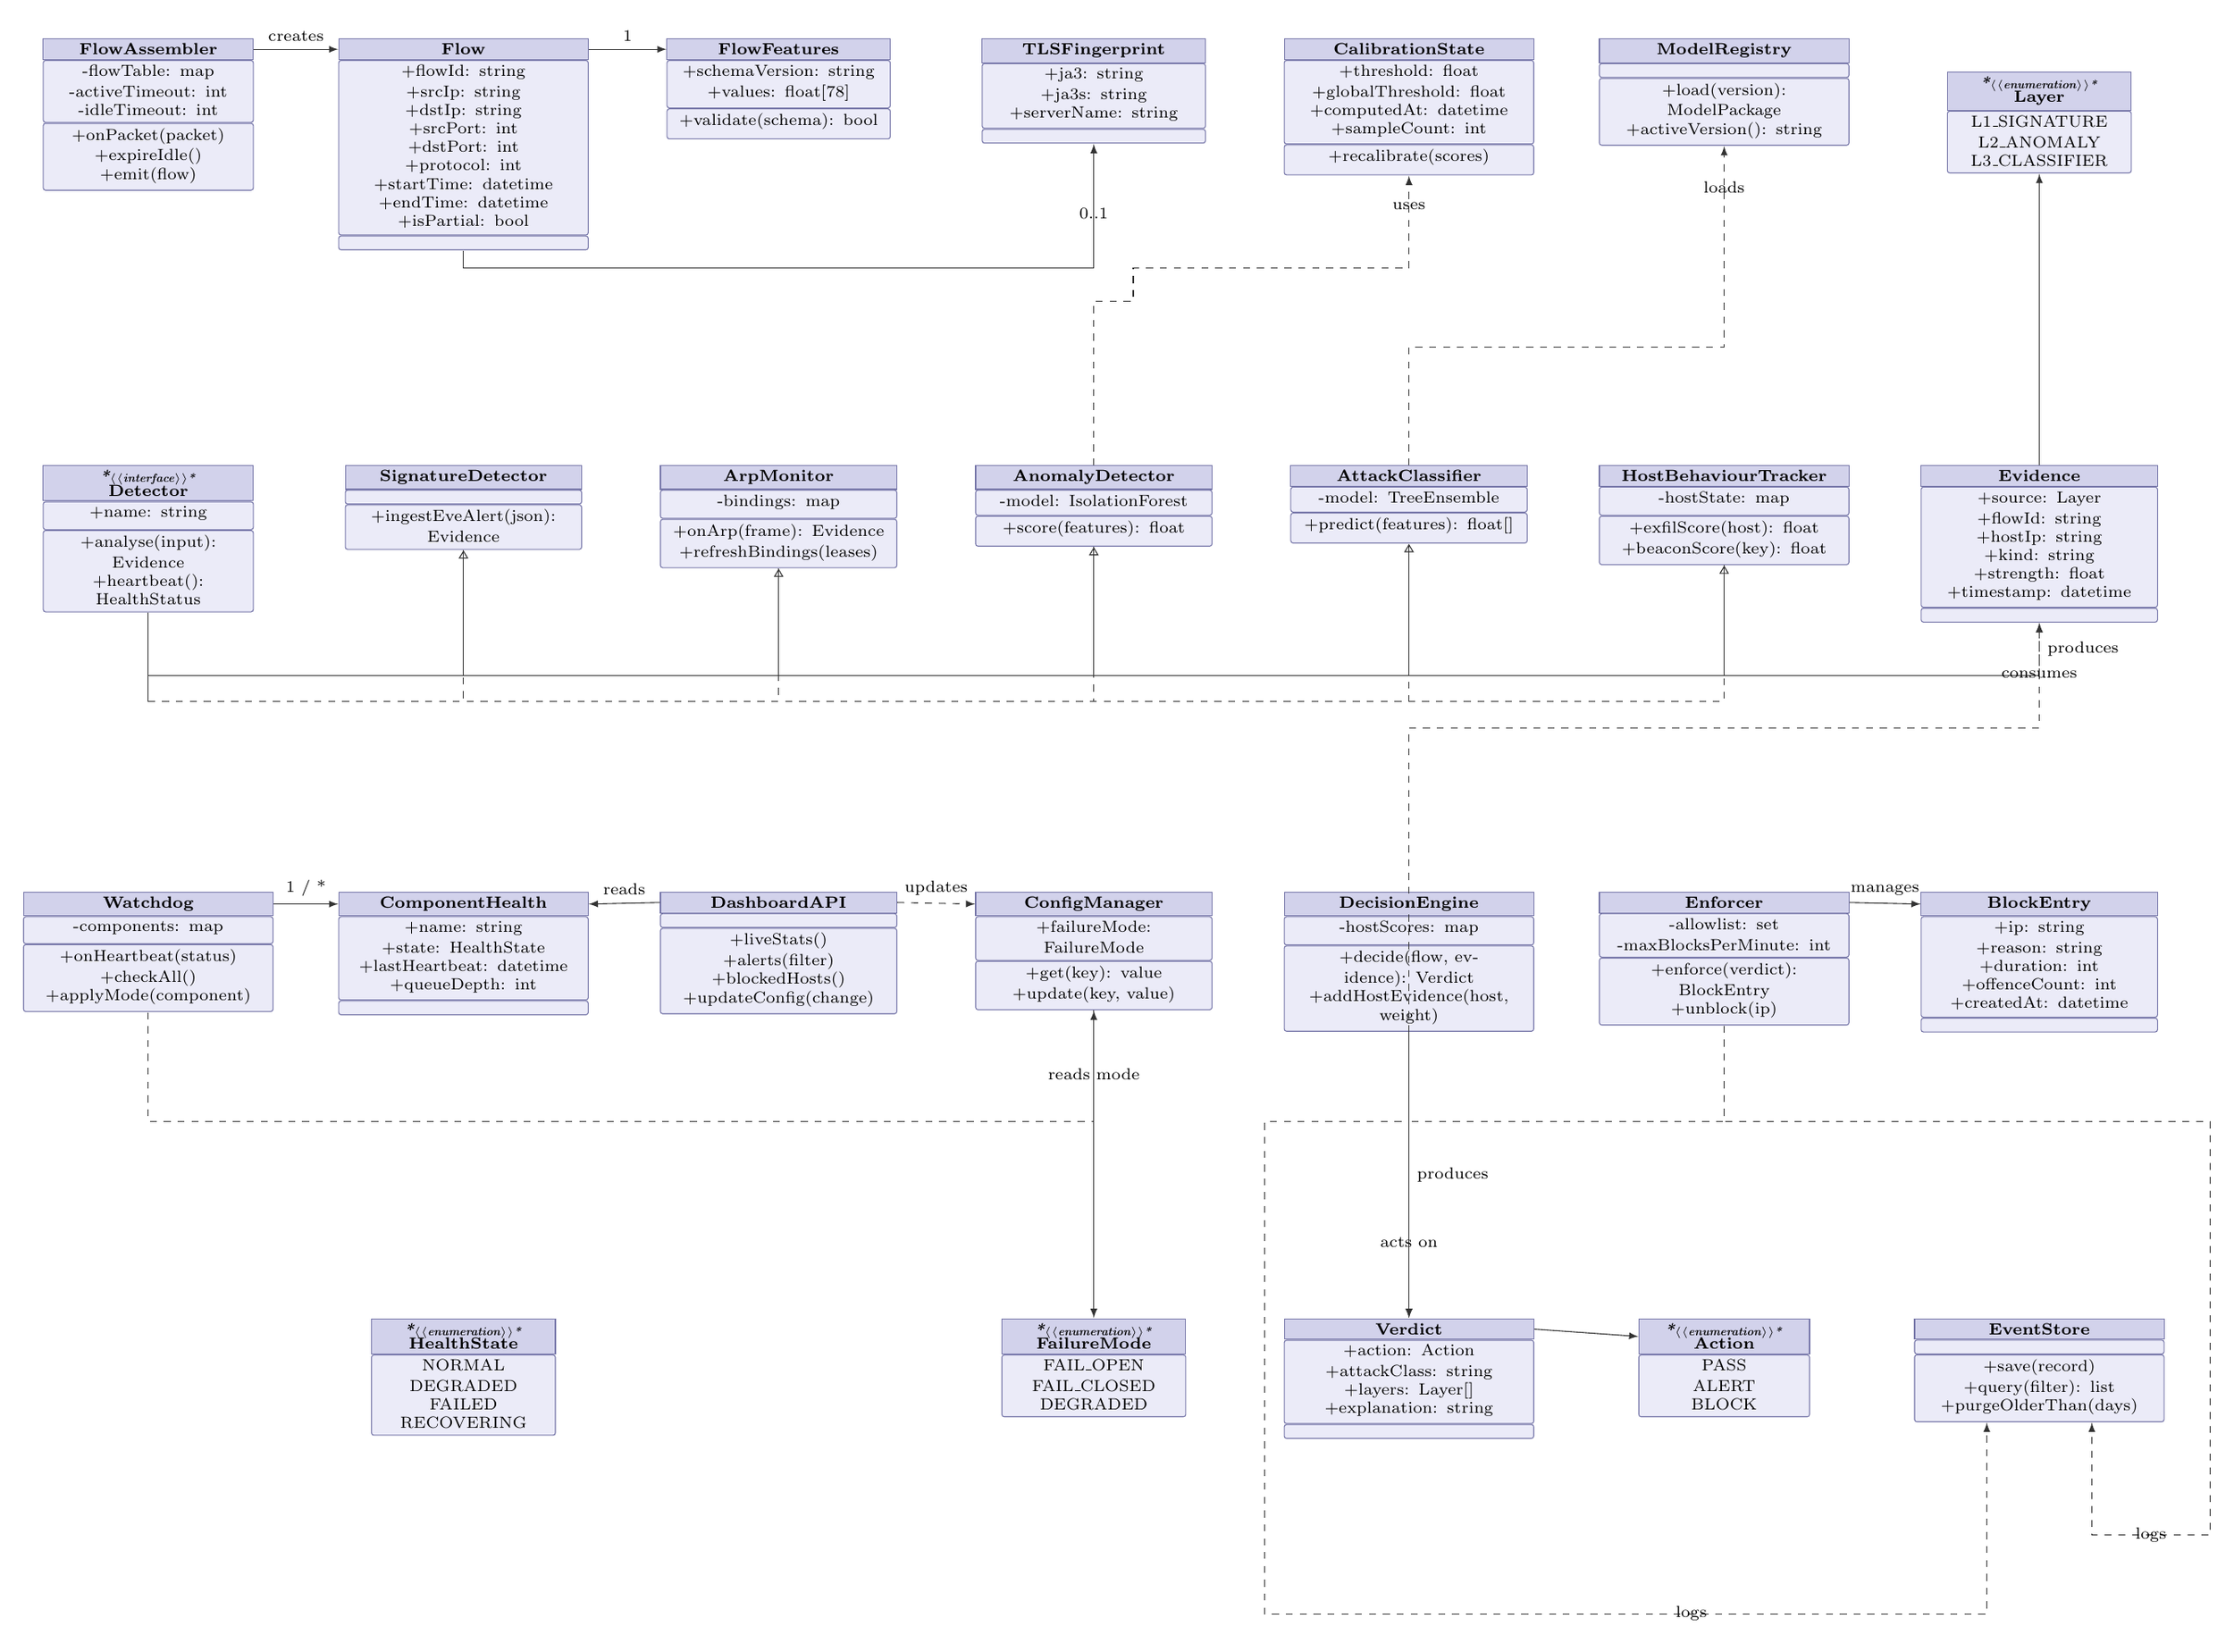
\begin{tikzpicture}[font=\scriptsize]
%% =====================================================================
%% GRID & CORRIDOR DEFINITION
%% Columns: x = 0, 4.8, 9.6, 14.4, 19.2, 24.0, 28.8
%% Rows:    y = 0, -6.5, -13.0, -19.5
%% Corridors (Empty horizontal lanes for routing):
%%   C1: y = 2.0   (Above Row 1)
%%   C2: y = -3.5  (Between Row 1 & 2)
%%   C3: y = -10.0 (Between Row 2 & 3)
%%   C4: y = -16.5 (Between Row 3 & 4)
%%   C5: y = -23.0 (Below Row 4)
%% =====================================================================
%% ---------- ROW 1 ----------
\umlNode{FA}{0,0}{3.2cm}{FlowAssembler}%
  {-flowTable: map\\-activeTimeout: int\\-idleTimeout: int}%
  {+onPacket(packet)\\+expireIdle()\\+emit(flow)}
\umlNode{FL}{4.8,0}{3.8cm}{Flow}%
  {+flowId: string\\+srcIp: string\\+dstIp: string\\+srcPort: int\\+dstPort: int\\+protocol: int\\+startTime: datetime\\+endTime: datetime\\+isPartial: bool}%
  {}
\umlNode{FF}{9.6,0}{3.4cm}{FlowFeatures}%
  {+schemaVersion: string\\+values: float[78]}%
  {+validate(schema): bool}
\umlNode{TLS}{14.4,0}{3.4cm}{TLSFingerprint}%
  {+ja3: string\\+ja3s: string\\+serverName: string}%
  {}
\umlNode{CS}{19.2,0}{3.8cm}{CalibrationState}%
  {+threshold: float\\+globalThreshold: float\\+computedAt: datetime\\+sampleCount: int}%
  {+recalibrate(scores)}
\umlNode{MR}{24.0,0}{3.8cm}{ModelRegistry}%
  {}%
  {+load(version): ModelPackage\\+activeVersion(): string}
\umlEnumBody{LayerEnum}{28.8,-0.5}{2.8cm}{Layer}%
  {L1\_SIGNATURE\\L2\_ANOMALY\\L3\_CLASSIFIER}
%% ---------- ROW 2 ----------
\umlInterface{DET}{0,-6.5}{3.2cm}{Detector}%
  {+name: string}%
  {+analyse(input): Evidence\\+heartbeat(): HealthStatus}
\umlNode{SIG}{4.8,-6.5}{3.6cm}{SignatureDetector}%
  {}%
  {+ingestEveAlert(json): Evidence}
\umlNode{ARP}{9.6,-6.5}{3.6cm}{ArpMonitor}%
  {-bindings: map}%
  {+onArp(frame): Evidence\\+refreshBindings(leases)}
\umlNode{AND}{14.4,-6.5}{3.6cm}{AnomalyDetector}%
  {-model: IsolationForest}%
  {+score(features): float}
\umlNode{ATC}{19.2,-6.5}{3.6cm}{AttackClassifier}%
  {-model: TreeEnsemble}%
  {+predict(features): float[]}
\umlNode{HBT}{24.0,-6.5}{3.8cm}{HostBehaviourTracker}%
  {-hostState: map}%
  {+exfilScore(host): float\\+beaconScore(key): float}
\umlNode{EV}{28.8,-6.5}{3.6cm}{Evidence}%
  {+source: Layer\\+flowId: string\\+hostIp: string\\+kind: string\\+strength: float\\+timestamp: datetime}%
  {}
%% ---------- ROW 3 ----------
\umlNode{WD}{0,-13.0}{3.8cm}{Watchdog}%
  {-components: map}%
  {+onHeartbeat(status)\\+checkAll()\\+applyMode(component)}
\umlNode{CH}{4.8,-13.0}{3.8cm}{ComponentHealth}%
  {+name: string\\+state: HealthState\\+lastHeartbeat: datetime\\+queueDepth: int}%
  {}
\umlNode{DA}{9.6,-13.0}{3.6cm}{DashboardAPI}%
  {}%
  {+liveStats()\\+alerts(filter)\\+blockedHosts()\\+updateConfig(change)}
\umlNode{CM}{14.4,-13.0}{3.6cm}{ConfigManager}%
  {+failureMode: FailureMode}%
  {+get(key): value\\+update(key, value)}
\umlNode{DE}{19.2,-13.0}{3.8cm}{DecisionEngine}%
  {-hostScores: map}%
  {+decide(flow, evidence): Verdict\\+addHostEvidence(host, weight)}
\umlNode{EN}{24.0,-13.0}{3.8cm}{Enforcer}%
  {-allowlist: set\\-maxBlocksPerMinute: int}%
  {+enforce(verdict): BlockEntry\\+unblock(ip)}
\umlNode{BE}{28.8,-13.0}{3.6cm}{BlockEntry}%
  {+ip: string\\+reason: string\\+duration: int\\+offenceCount: int\\+createdAt: datetime}%
  {}
%% ---------- ROW 4 ----------
\umlEnumBody{HSEnum}{4.8,-19.5}{2.8cm}{HealthState}%
  {NORMAL\\DEGRADED\\FAILED\\RECOVERING}
\umlEnumBody{FMEnum}{14.4,-19.5}{2.8cm}{FailureMode}%
  {FAIL\_OPEN\\FAIL\_CLOSED\\DEGRADED}
\umlNode{VD}{19.2,-19.5}{3.8cm}{Verdict}%
  {+action: Action\\+attackClass: string\\+layers: Layer[]\\+explanation: string}%
  {}
\umlEnumBody{ActionEnum}{24.0,-19.5}{2.6cm}{Action}%
  {PASS\\ALERT\\BLOCK}
\umlNode{EST}{28.8,-19.5}{3.8cm}{EventStore}%
  {}%
  {+save(record)\\+query(filter): list\\+purgeOlderThan(days)}
%% =====================================================================
%% RELATIONSHIPS & ROUTING
%% All routes use horizontal/vertical segments and stay in the gaps
%% between rows or in the clear space below the diagram.
%% =====================================================================
%% --- ROW 1 INTERNAL ---
\draw[assoc] (FA-head.east) -- node[above,font=\scriptsize]{creates} (FL-head.west);
\draw[compose] (FL-head.east) -- node[above,font=\scriptsize]{1} (FF-head.west);
%% Flow -> TLSFingerprint: route through the gap between rows 1 and 2.
\draw[assoc] (FL.south) -- (4.8,-3.5) -- (14.4,-3.5) -- (TLS.south)
    node[pos=0.55,below,font=\scriptsize]{0..1};
%% --- ROW 2 / TOP-ROW DEPENDENCIES ---
%% AnomalyDetector -> CalibrationState.
\draw[dep] (AND-head.north) -- (14.4,-4.0) -- (15.0,-4.0) -- (15.0,-3.5) -- (19.2,-3.5) -- (CS.south)
    node[pos=0.55,above,font=\scriptsize]{uses};
%% AttackClassifier -> ModelRegistry.
\draw[dep] (ATC-head.north) -- (19.2,-4.7) -- (24.0,-4.7) -- (24.0,-3.5) -- (MR.south)
    node[pos=0.55,above,font=\scriptsize]{loads};
%% --- DETECTOR INTERFACE REALIZATION ---
%% The shared bus is below row 2; each arrow enters at the bottom edge
%% of its target class, rather than passing through the class body.
\coordinate (detBus) at (0,-10.1);
\draw[line] (DET.south) -- (detBus);
\foreach \target in {SIG,ARP,AND,ATC,HBT}{
    \draw[realize] (detBus) -| (\target.south);
}
%% --- DETECTORS -> EVIDENCE ---
%% A dedicated horizontal lane below row 2.
\coordinate (evBus) at (28.8,-9.7);
\draw[line] (0,-9.7) -- (28.8,-9.7);
\foreach \src in {SIG,ARP,AND,ATC,HBT}{
    \draw[line] (\src.south) -- (\src.south |- evBus);
}
\draw[dep] (evBus) -- (EV.south)
    node[midway,right,font=\scriptsize]{produces};
%% Evidence -> Layer enumeration (vertical, in the rightmost column).
\draw[assoc] (EV.north) -- (LayerEnum.south);
%% --- ROW 3 INTERNAL ---
\draw[assoc] (WD-head.east) -- node[above,font=\scriptsize]{1 / *} (CH-head.west);
\draw[assoc] (DA-head.west) -- node[above,font=\scriptsize]{reads} (CH-head.east);
%% Watchdog -> ConfigManager: route below row 3, then enter at its bottom.
\draw[dep] (WD.south) -- (0,-16.5) -- (14.4,-16.5) -- (CM.south)
    node[pos=0.55,below,font=\scriptsize]{reads mode};
%% DashboardAPI -> ConfigManager.
\draw[dep] (DA-head.east) -- node[above,font=\scriptsize]{updates} (CM-head.west);
%% ConfigManager -> FailureMode.
\draw[assoc] (CM.south) -- (FMEnum.north);
%% DecisionEngine -> Verdict.
\draw[assoc] (DE.south) -- node[right,font=\scriptsize]{produces} (VD.north);
%% Enforcer -> BlockEntry.
\draw[assoc] (EN-head.east) -- node[above,font=\scriptsize]{manages} (BE-head.west);
%% Verdict -> Action enumeration.
\draw[assoc] (VD-head.east) -- (ActionEnum-head.west);
%% Enforcer -> Verdict: route through the gap between rows 3 and 4.
\draw[dep] (EN.south) -- (24.0,-16.5) -- (19.2,-16.5) -- (VD.north)
    node[pos=0.55,below,font=\scriptsize]{acts on};
%% --- CROSS-ROW DEPENDENCIES ---
%% DecisionEngine -> Evidence: use a separate lane in the row gap.
\draw[dep] (DE.south) -- (19.2,-10.5) -- (28.8,-10.5) -- (EV.south)
    node[pos=0.62,below,font=\scriptsize]{consumes};
%% Enforcer -> EventStore: leave row 3 through the C4 corridor,
%% then descend outside the right edge of the row-4 classes.
\draw[dep] (EN.south) -- (24.0,-16.5) -- (31.4,-16.5)
    -- (31.4,-22.8) -- (29.6,-22.8)
    -- ($(EST.south)+(0.8,0)$);
\node[font=\scriptsize] at (30.5,-22.8) {logs};

%% DecisionEngine -> EventStore: leave row 3 through C4, pass
%% outside the left edge of Verdict, and use a separate lower lane.
\draw[dep] (DE.south) -- (19.2,-16.5) -- (17.0,-16.5)
    -- (17.0,-24.0) -- (28.0,-24.0)
    -- ($(EST.south)+(-0.8,0)$);
\node[font=\scriptsize] at (23.5,-24.0) {logs};

\end{tikzpicture}

}

\end{center}

\end{document}